\documentclass[laboratorio]{guia}

\def \practnum {10}
\def \practica {Polarizaci\'on}
% \def \practica {Polarizaci\'on de la luz}

\def \materia {Laboratorio de F\'\i sica II para Qu\'\i micos}
\def \periodo {2do. Cuatrimestre de 2015}
\def \catedra {Pablo Cobelli}
\def \website {http://materias.df.uba.ar/f2qa2015c2}

\usepackage{graphics}
\usepackage{amsmath}
\usepackage{amsfonts}
\usepackage{graphicx}
\usepackage{float}
\usepackage{wrapfig}
\usepackage{subfigure}
\usepackage{bm}
\usepackage{grffile}
\usepackage{color}
\usepackage{framed}
\usepackage[utf8]{inputenc}
\usepackage[T1]{fontenc}
\usepackage{lmodern}
\usepackage{circuitikz}
\usepackage[spanish]{babel}
\usepackage{babelbib}
\selectbiblanguage{spanish}



%----------------------------------------------------------
% Agrega al path de figuras el subdirectorio con el mismo
%     nombre que el archivo principal del proyecto
\graphicspath{{./\jobname/}}

%----------------------------------------------------------
% Definicion del entorno 'sabermas'
\makeatletter
\definecolor{shadecolor}{rgb}{0.89,0.91,0.94}
\newenvironment{sabermas}[1]{%
\vfill
\begin{shaded}
  \begin{center}
  {\textsection{Para saber m\'as}}
  \end{center}
  #1
\sf } 
{%
\end{shaded}%
}
\makeatother

%----------------------------------------------------------
% Definicion del entorno 'problema'
\newcounter{ContadorProblema}
\setcounter{ContadorProblema}{0}
\newcounter{TieneFiguraAsociada}
\setcounter{TieneFiguraAsociada}{0}
\newcounter{UbicacionFigura}
\setcounter{UbicacionFigura}{0}

\newenvironment{problema}[2][]
{%
    \ifx\relax#1\relax%
        \setcounter{TieneFiguraAsociada}{0}
        \else
        \setcounter{TieneFiguraAsociada}{1}
    \fi
    \def \archivofigura {#1}
    % 
    \refstepcounter{ContadorProblema}
    \noindent%
    \ifnum\value{TieneFiguraAsociada} < 1%
        {\sffamily \bfseries Problema \arabic{ContadorProblema}.}
        %{\sc {#1}}%
        \par\nobreak\par\nobreak%
        \medskip 
    \else
        % Va con figura; resta determinar de que lado.
        \ifnum\value{UbicacionFigura} < 1
            % Poner la figura del lado derecho
            \begin{minipage}{12.25cm}
            {\sffamily \bfseries Problema \arabic{ContadorProblema}.}
            %{\sc {#1}}%
            \par\nobreak\par\nobreak%
            \medskip 
        \else
            % Poner la figura del lado izquierdo
            \begin{minipage}{4.5cm}
                \centering
                \includegraphics[width=4.5cm]{\archivofigura}
                {\footnotesize {\sffamily Esquema asociado al 
                problema \arabic{ContadorProblema}}.}
            \end{minipage}\hfill%
            \begin{minipage}{12.25cm}
                {\sffamily \bfseries Problema \arabic{ContadorProblema}.}
                %{\sc {#1}}%
                \par\nobreak\par\nobreak%
                \medskip 
        \fi
    \fi
}
{%
    \ifnum\value{TieneFiguraAsociada} < 1%
        % \par \bigskip \vskip 0.3cm
    \else
        % Va con figura; resta determinar de que lado.
        \ifnum\value{UbicacionFigura} < 1
            % Poner la figura del lado derecho
            \end{minipage}\hfill%
            \begin{minipage}{4.5cm}
                \centering
                \includegraphics[width=4.5cm]{\archivofigura}
                {\footnotesize {\sffamily Esquema asociado al 
                problema \arabic{ContadorProblema}}.}
            \end{minipage}
        \else
            % Poner la figura del lado izquierdo
            \end{minipage}%
        \fi
    \fi
    \setcounter{TieneFiguraAsociada}{0}
    \par \bigskip \vskip 0.3cm
    % Permutamos el valor de la ubicacion
    \ifnum\value{UbicacionFigura} < 1
        \setcounter{UbicacionFigura}{1}
    \else
        \setcounter{UbicacionFigura}{0}
    \fi
}

%----------------------------------------------------------
% Definicion/Redefinicion de estilos
\renewcommand{\vec}[1]{\ensuremath{\mathbf{#1}}}


\hyphenation{ coe-fi-cien-tes coe-fi-cien-te au-to-va-lor
              au-to-va-lo-res co-rres-pon-der pro-ble-ma 
              cual-quie-ra po-la-ri-za-cio-nes }

\graphicspath{{./polarizacion/}}

\begin{document}
\objetivo{
  Determinar experimentalmente:
  (a) la intensidad lumínica transmitida a través de un polarizador lineal, en función de la orientación, y
  (b) el índice de refracción de un medio empleando el ángulo de Brewster.
  \tematicas{Polarización, Ley de Malus, polarización por reflexión, ángulo de Brewster.}
  }
\maketitle


\section{Introducción}

En una onda transversal la propiedad que vibra u oscila es una magnitud de carácter vectorial y lo hace en una dirección perpendicular a la de propagación.
Decimos que una onda transversal está polarizada si la propiedad que vibra lo hace de un modo predecible, es decir, siempre paralelamente a una direccián fija (polarización lineal) o con el vector que describe la vibración rotando a una frecuencia dada alrededor de la dirección de propagación (polarización circular).
Un ejemplo de onda mecánica transversal es el caso de una onda viajando por una cuerda; aquí el desplazamiento o elongación es perpendicular a dirección de propagación de la onda.
La vibración puede ocurrir en cualquier dirección perpendicular a su propagación. Si se intercala una rejilla en algún punto de la cuerda, es claro que sólo las oscilaciones en la dirección de las rejas podrán pasar.
Este dispositivo, que deja pasar únicamente las vibraciones en un solo estado de polarización se denomina \emph{polarizador}.


\section{Polarización por reflexión}

Usando un láser, un polarímetro y el fotómetro, estudie las características de polarización de un haz láser.
¿Es polarizada la luz de un láser de estado sólido?
¿Y la de un láser de He-Ne?
Para el láser que está estudiando, si la luz es polarizada linealmente, determine la dirección de polarización.

\begin{figure}[ht]
  \centering
  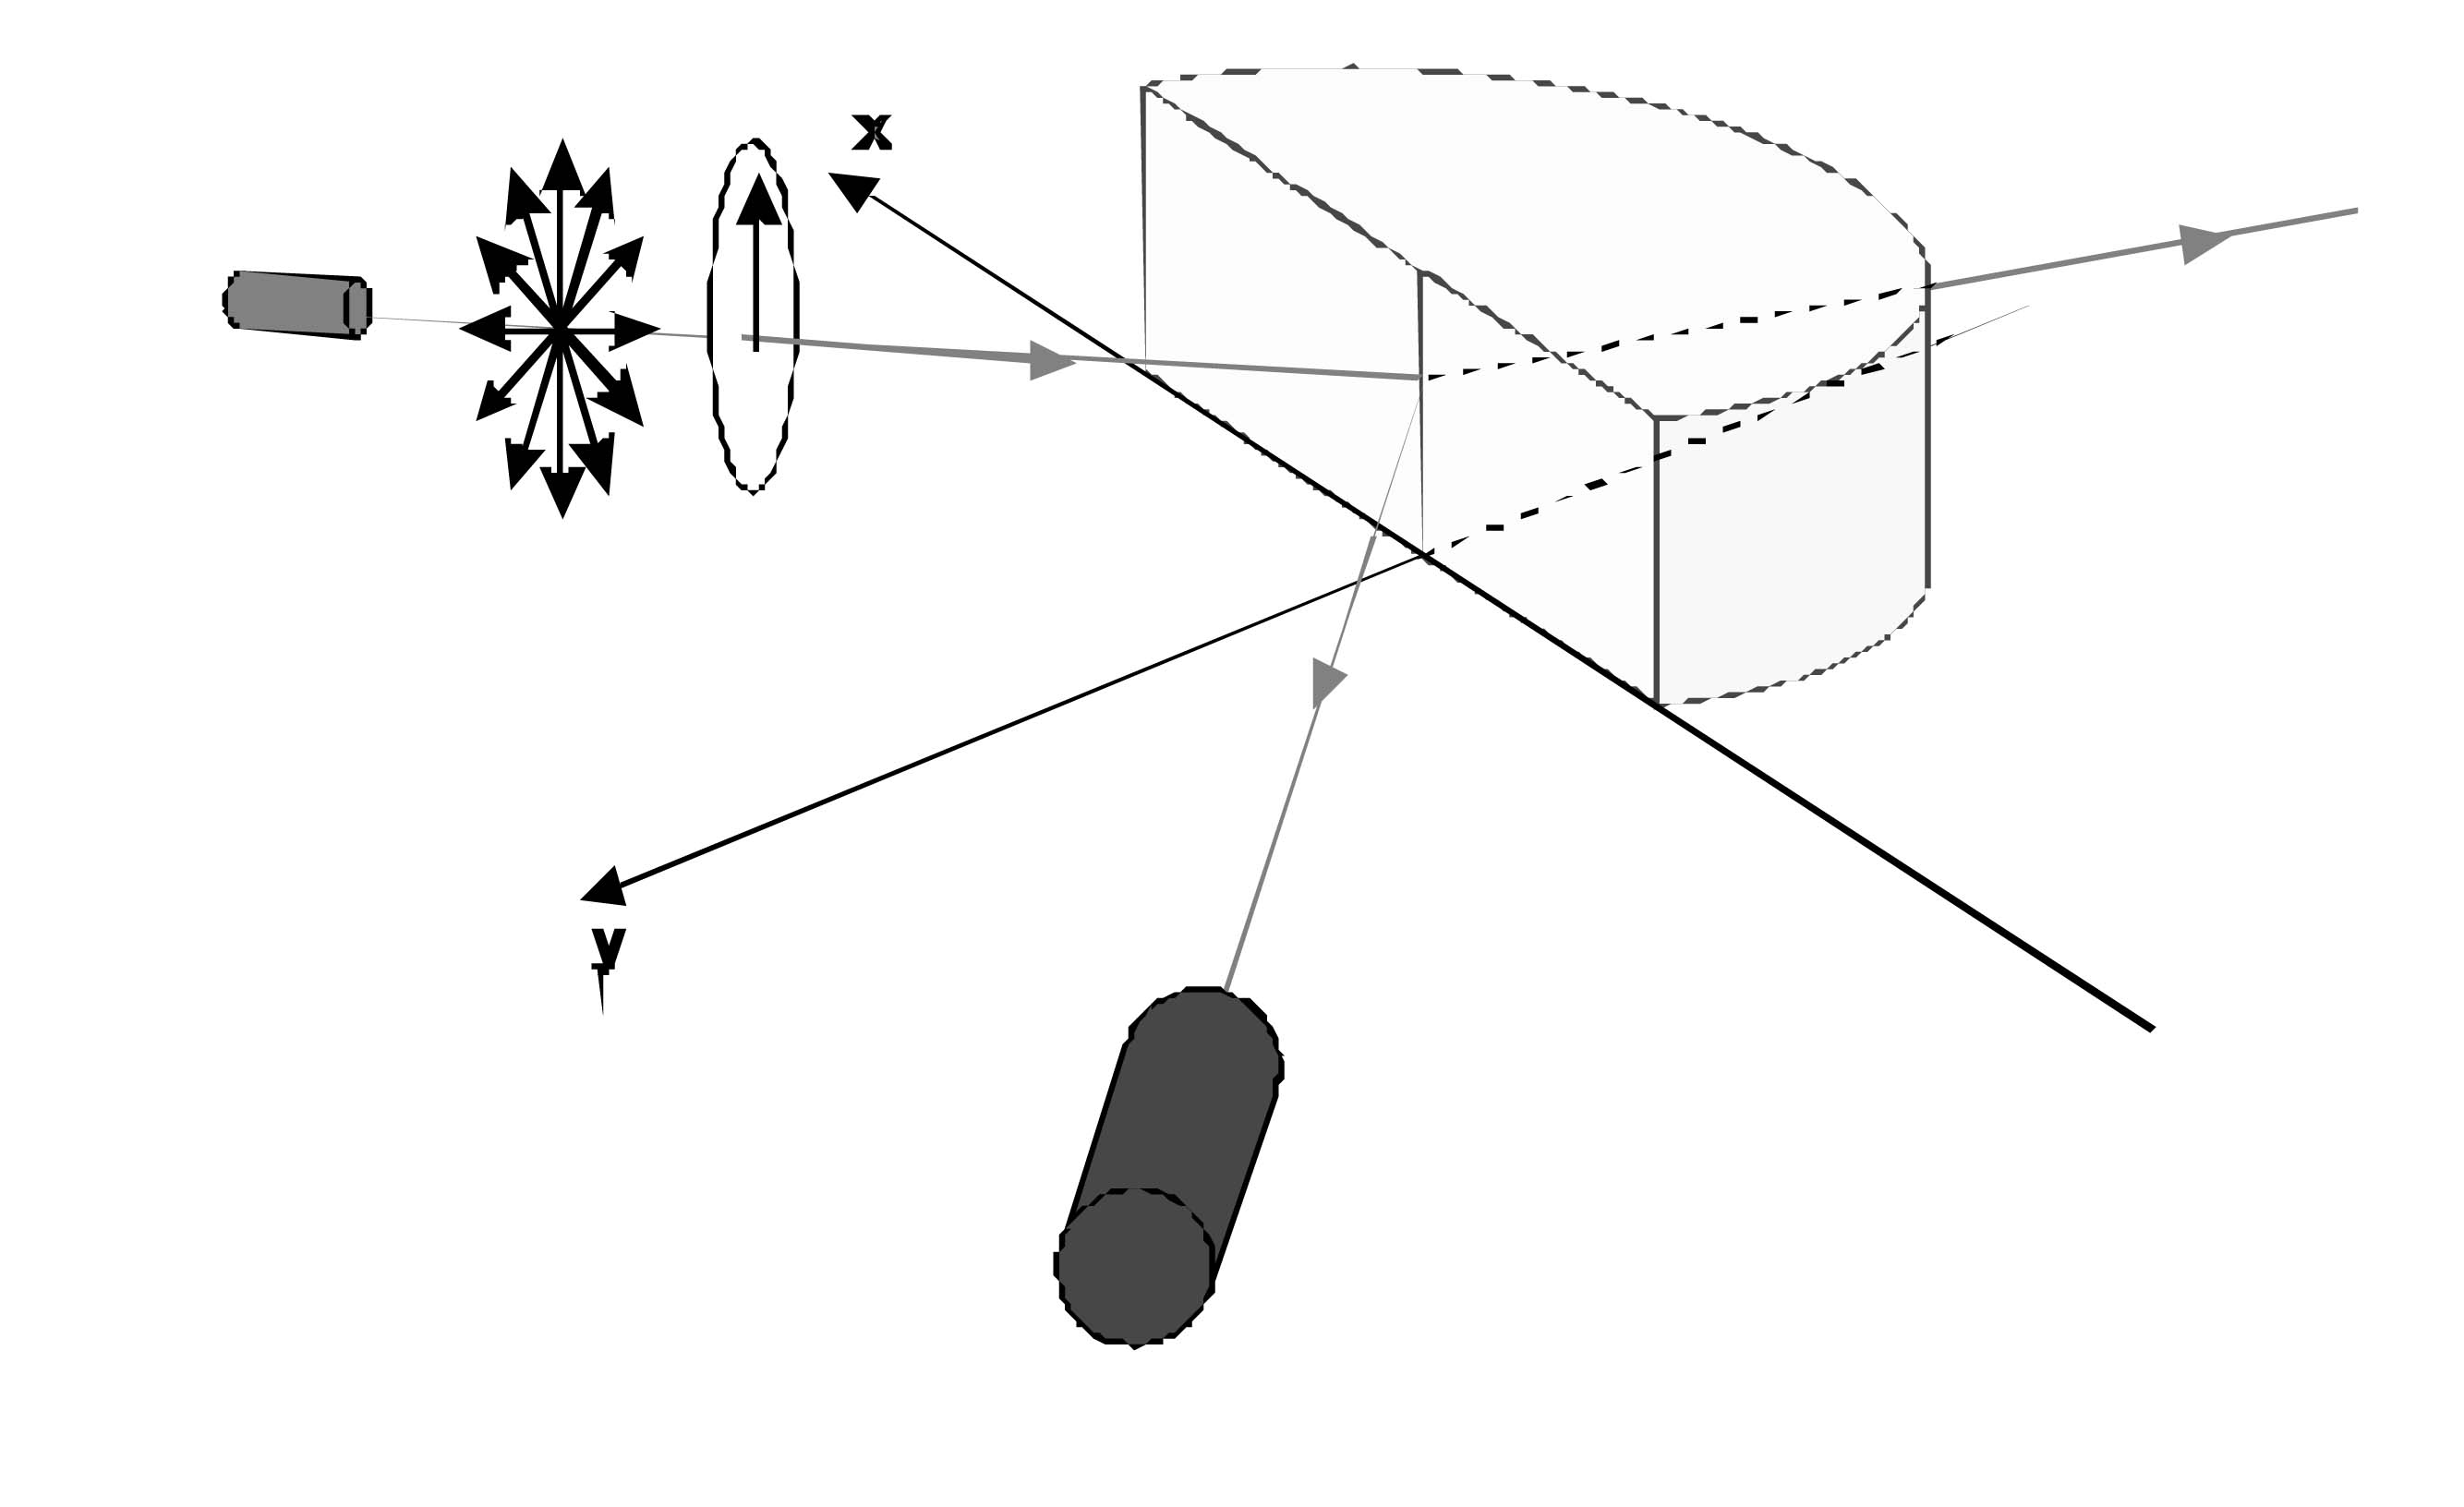
\includegraphics[width=8.5cm]{LG12--001.png}
  \caption{Esquema experimental propuesto para el estudio de la polarización por reflexión.}
  \label{fig:2}
\end{figure}

Usando el dispositivo esquemátizado en la figura \ref{fig:2}, estudie cómo varía la intensidad de la luz reflejada y transmitida por una muestra de vidrio o acrílico.
Para esta parte de la guía, es conveniente que la muestra no sea de caras paralelas.
De este modo los haces reflejados y transmitidos por la segunda cara no llegarán al detector o pantalla, proveniendo sólo de la reflexión y transmisión en una sola cara.
Realice este estudio usando un haz láser polarizado, con el campo eléctrico oscilando: (a) en un plano perpendicular al plano de reflexión (modo S) y (b) en la dirección de dicho plano (modo P).

Empleando ahora un dispositivo similar al indicado en la misma figura, estudie los estados de polarización de los rayos transmitidos y reflejados, para la situación especial en la cual el rayo reflejado y el transmitido forman un ángulo de \(\pi/2\)~rad.
Determine el ángulo de reflexión y, a partir de este dato, estime el índice de refracción del material. 
Discuta y explique sus resultados acerca del estado de polarización de los rayos reflejados y transmitidos.
Sugerencia: para esta parte puede ser conveniente usar un láser con su plano de polarización formando un ángulo de aproximadamente \(\pi/4\)~rad respecto a la perpendicular al plano de reflexión.
En otras palabras, el láser deberá tener una componente S y otra P de magnitudes comparables.


\section{Ley de Malus}
Estudie cómo varía la intensidad de luz que recibe el detector en función del ángulo entre dos polarizadores lineales empleando el dispositivo experimental se muestra esquem\'aticamente en la Fig. \ref{fig:Malus}.

\begin{figure}[ht]
  \centering
  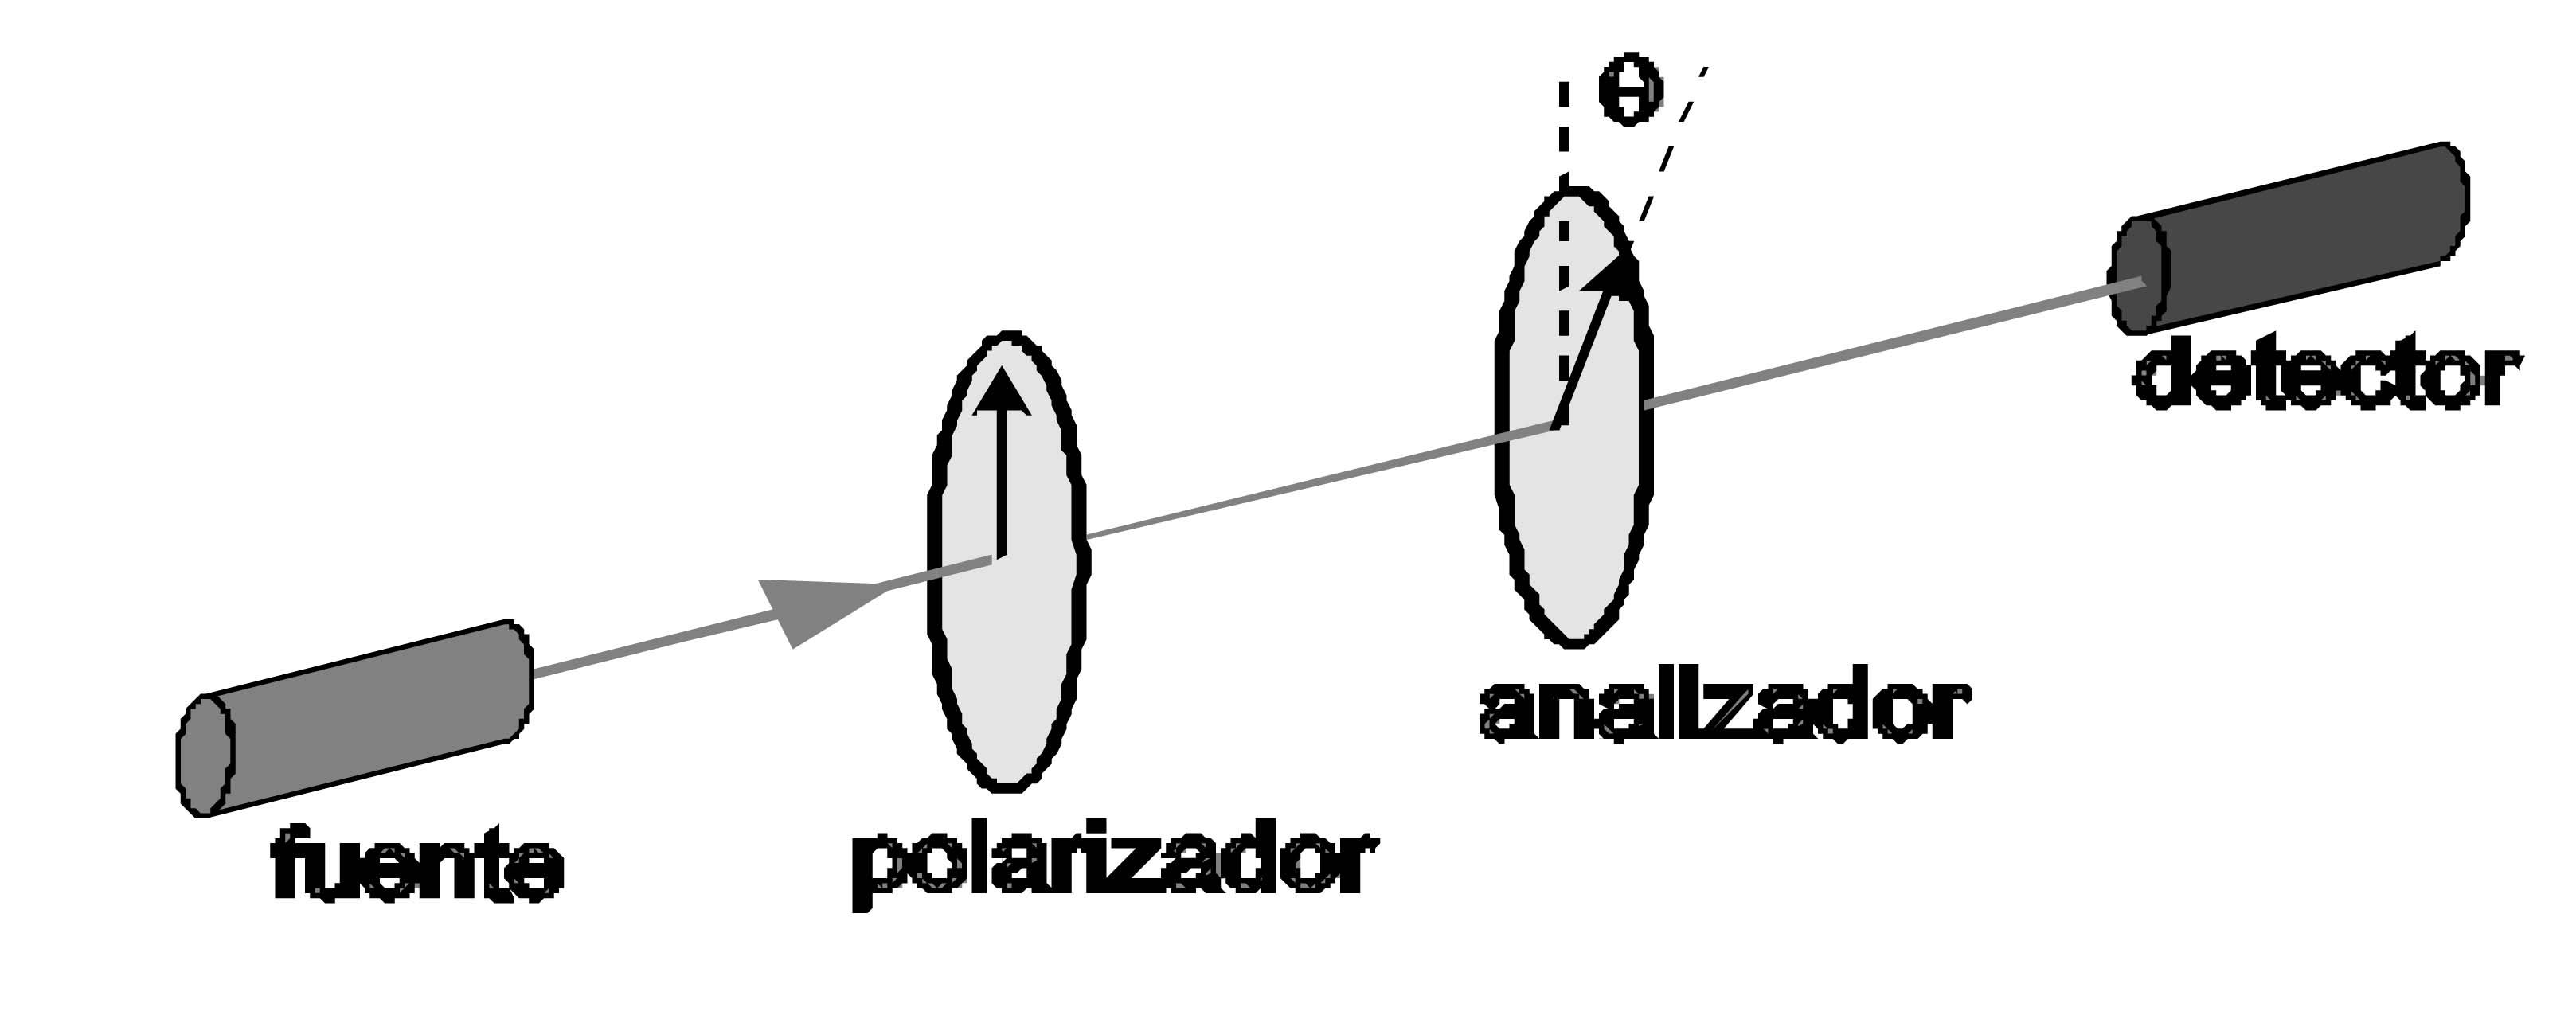
\includegraphics[width=8.5cm]{LG12--000.png}
  \caption{Esquema experimental propuesto para el estudio de la ley de Malus.}
  \label{fig:Malus}
\end{figure}

La fuente de luz es una lámpara incandescente y el detector, un fotómetro.
El primer polarizador (cercano a la fuente) se denomina simplemente polarizador y el más alejado es el \emph{analizador}.
Este último deberá tener un goniómetro para medir su posición angular relativa a la del polarizador (\(theta\)).


\subsection{Actividad óptica}
Ciertas moléculas poseen una estructura quiral, y dependiendo que estereoisómero sea dominante, estando en solución producen la rotación del plano de polarización de la luz que atraviese esta última.
Tal es el caso de la Sacarosa en solución acuosa que presenta una \emph{rotación específica} de \SI{+66,37}{\degree\cubic\centi\metre\per\deci\metre\per\gram}.

Para este ensayo usualmente se ubica la solución en un contenedor cilíndrico con caras planas transparente de una longitud de \SI{1}{\deci\metre}, de ahí que la rotación específica se indique en función de esta unidad, y de la concentración de la solución en \si{\gram\per\cubic\centi\metre}.

Si dispone de tal contenedor fabrique una solución de una concentración conocida y verifique con el dispositivo con que estudió la Ley de Malus que se produce la rotación del plano de polarización en el grado esperado.
De interponer el contenedor notará que el mínimo (o máximo de transmisión) lo encontrará rotando el analizador un ángulo adicional respecto al que lo ubicada cuando no se encontraba el contenedor para obtener el mismo efecto.
Tal diferencia en \(theta\) deberá corresponderse con la concentración de la solución.



\nocite{Alonso1998,Hecht1986,Jenkins2001}
\bibliographystyle{unsrt} 
\bibliography{Bibliografia}

\end{document}
